\documentclass[spanish,letterpaper,oneside]{article}

% Datos del documento
\def\documenttitle {Desarrollos planos y áreas de cuerpos geométricos}
\def\documentsubtitle {Temas selectos de matemáticas I}
\def\documentsubject {Actividad 7 · Ficha y secuencia para exposición}
\def\documentauthor {Mtro. Martín Jonathan de la Cruz Muñoz}
\def\coursename {Temas selectos de matemáticas I}
\def\coursecode {PFM02}

% Identidad institucional
\def\universityname {Instituto de Investigación, Innovación y Estudios de Posgrado para la Educación del Estado de Nuevo León}
\def\universityfaculty {Maestría en Aprendizaje y Enseñanza de las Matemáticas}
\def\universitydepartment {Temas selectos de matemáticas I}
\def\universitydepartmentimage {img/iiiepe/marca-iiiepe.png}
\def\universitydepartmentimagecfg {height=1.75cm}
\def\universitylocation {Monterrey, Nuevo León}
\def\studentfullname {Mtro. Martín Jonathan de la Cruz Muñoz}
\def\studentid {00874}
\def\studentemail {martin.delacruz@campus.iiiepe.edu.mx}
\def\programperiod {1er tetramestre, marzo--julio de 2026}
\def\programmodality {Modalidad presencial}
\def\programshort {MAEM}

\def\authortable {
  \begin{tabular}{ll}
    \textbf{Alumno:} & \studentfullname \\
    Matrícula: & \studentid \\
    Correo institucional: & \studentemail \\
    Unidad: & \coursename \\
    Programa: & \programshort \\
    Periodo: & \programperiod \\
    & \\
    \multicolumn{2}{l}{Fecha de realización: 13 de octubre de 2026} \\
    \multicolumn{2}{l}{\universitylocation}
  \end{tabular}
}

\input{template}

\usepackage{helvet}
\renewcommand{\familydefault}{\sfdefault}
\usepackage{array}
\usepackage{longtable}
\usepackage{pdflscape}
\usepackage{tikz}
\usepackage[most]{tcolorbox}
\usetikzlibrary{arrows.meta,positioning,calc,fit,backgrounds}

\definecolor{iiiepeNavy}{HTML}{163B5C}
\definecolor{iiiepeBlue}{HTML}{1F6F9F}
\definecolor{iiiepeAqua}{HTML}{20B7A8}
\definecolor{iiiepeOrange}{HTML}{F28C28}
\definecolor{iiiepePaper}{HTML}{F6F8F7}
\definecolor{iiiepeInk}{HTML}{1E2A32}
\def\portraittitlecolor {iiiepeNavy}
\setcitestyle{authoryear,open={(},close={)}}

\newcommand{\insertcoverwatermark}{%
  \AddToShipoutPictureBG*{%
    \begin{tikzpicture}[remember picture,overlay]
      \node[opacity=.09,inner sep=0pt] at (current page.center)
      {\includegraphics[width=.58\paperwidth]{img/iiiepe/logo-puntos.png}};
    \end{tikzpicture}%
  }%
}

\newtcolorbox{reportelecturabox}[1][]{%
  enhanced,breakable,
  colback=iiiepePaper,colframe=iiiepeNavy,
  boxrule=1pt,leftrule=4pt,arc=2pt,
  left=8pt,right=8pt,top=6pt,bottom=6pt,
  before skip=6pt,after skip=10pt,
  fonttitle=\bfseries\color{white},coltitle=white,
  colbacktitle=iiiepeNavy,
  attach boxed title to top left={xshift=8pt,yshift=-2pt},
  boxed title style={colback=iiiepeNavy,colframe=iiiepeNavy,arc=1pt},
  title={Reporte de lectura},#1}

\newtcolorbox{fichalecturabox}[1][]{%
  enhanced,breakable,
  colback=iiiepeAqua!7,colframe=iiiepeAqua!70!iiiepeNavy,
  boxrule=.6pt,arc=1pt,
  left=7pt,right=7pt,top=4pt,bottom=4pt,
  fontupper=\small,before upper={\setstretch{1.0}},
  fonttitle=\bfseries\color{iiiepeNavy},coltitle=iiiepeNavy,
  colbacktitle=iiiepeAqua!7,
  title={Ficha de la lectura},#1}



\usepackage{tabularx,colortbl,pgfplots,enumitem,needspace}\pgfplotsset{compat=1.18}\definecolor{iiiepePale}{HTML}{EEF5F8}
\setlength{\parskip}{5pt}\setlength{\parindent}{0pt}
\begin{document}\insertcoverwatermark\templatePortrait\templatePagecfg\templateFinalcfg\fancyfoot{}\fancyfoot[L]{\scriptsize IIIEPE · MAEM}\fancyfoot[C]{\scriptsize\thepage}\fancyfoot[R]{\scriptsize Actividad 7}\setstretch{1.3}\raggedbottom
\section{Reto y contenido matemático}
El reto propuesto es diseñar envases a partir de figuras planas y justificar el área de material. El contenido corresponde a construcción de cuerpos, sólidos de revolución, desarrollos planos y áreas laterales y totales de prismas y pirámides. En mis contextos de mantenimiento e ingeniería, la conexión con fabricación favorece la pertinencia, pero el aprendizaje debe incluir argumentación geométrica y acceso equitativo a herramientas.
\section{Fase 1 · Saberes de nuestra comunidad}
Compararía una caja y un envase cilíndrico: ¿qué figuras aparecen al abrirlos y qué medidas permiten estimar el material? La estimación inicial se contrasta con un dibujo, evitando sumar longitudes como si fueran áreas.
\section{Fase 2 · Indagación y diseño}
Un rectángulo que gira alrededor de uno de sus lados genera un cilindro; un triángulo rectángulo que gira alrededor de un cateto genera un cono; un semicírculo que gira alrededor de su diámetro genera una esfera. El desarrollo de un cilindro incluye dos círculos de radio $r$ y un rectángulo de altura $h$ y base $2\pi r$. El cono incluye un círculo y un sector de radio igual a la generatriz $g$, cuyo arco mide $2\pi r$; su ángulo es $360^\circ r/g$.
\begin{center}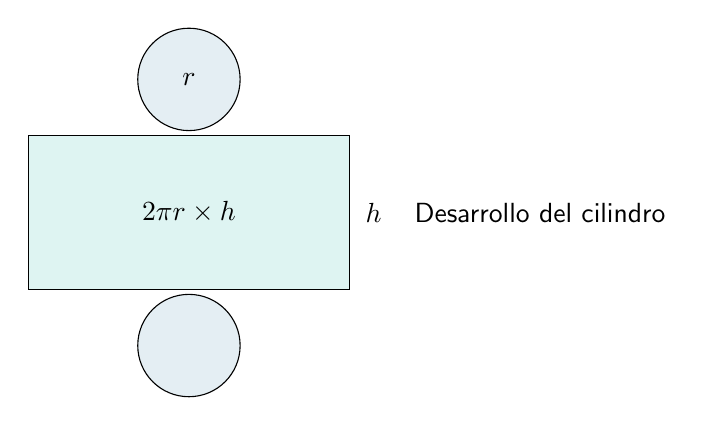
\begin{tikzpicture}[scale=.65]
\draw[fill=iiiepeAqua!15] (0,0) rectangle (6.28,3);\draw[fill=iiiepeBlue!12] (3.14,4.1) circle (1);\draw[fill=iiiepeBlue!12] (3.14,-1.1) circle (1);\node at (3.14,1.5){$2\pi r\times h$};\node[right] at (6.4,1.5){$h$};\node at (3.14,4.1){$r$};\node at (10,1.5){Desarrollo del cilindro};\end{tikzpicture}\end{center}
\section{Fase 3 · Resultados resueltos}
Para un prisma rectangular de $8\times5\times3$ cm, el área total es $2(8\cdot5+8\cdot3+5\cdot3)=158$ cm$^2$. Tomando base $8\times5$, el área lateral es $2(8+5)(3)=78$ cm$^2$ y el volumen es 120 cm$^3$.
Para un cilindro cerrado de radio 3 cm y altura 10 cm, $A_L=2\pi rh=60\pi$ cm$^2$ y $A_T=2\pi r(h+r)=78\pi\approx245.04$ cm$^2$. El volumen es $\pi r^2h=90\pi$ cm$^3$.
Para una pirámide regular de base cuadrada de lado 6 cm y altura 4 cm, el apotema lateral es $a=\sqrt{4^2+3^2}=5$ cm. El área lateral es $P_ba/2=(24)(5)/2=60$ cm$^2$; el total es $60+36=96$ cm$^2$ y el volumen es $(1/3)(36)(4)=48$ cm$^3$. El apotema no debe confundirse con la altura vertical.
Para un cono de radio 3 cm y altura 4 cm, $g=5$ cm; su desarrollo lateral es un sector de radio 5 cm y ángulo $216^\circ$. El área lateral es $\pi rg=15\pi$ cm$^2$ y el área total es $24\pi$ cm$^2$.
\section{Fase 4 · Comunicación del diseño}
Construiría los desarrollos con papel cuadriculado, marcaría pestañas por separado y compararía el área teórica con el material utilizado. Los cálculos anteriores son exactos para los cuerpos ideales; un envase real requiere tolerancias, espesor y desperdicio de corte. No se presentan como un prototipo ya fabricado.
\section{Comprobación de los desarrollos y de las unidades}
En el cilindro, el rectángulo debe tener base $2\pi r$, porque su borde rodea exactamente una circunferencia. Si se dibujara una base de longitud $2r$, el desarrollo no cerraría. En la pirámide regular, cada cara triangular tiene base 6 y altura inclinada 5; cuatro caras dan $4(6\cdot5/2)=60$ cm$^2$, coincidente con $P_ba/2$.
Para el cono del ejemplo, el sector tiene radio 5 y ángulo $216^\circ$. Su arco mide $(216/360)(2\pi\cdot5)=6\pi$, igual a la circunferencia de la base de radio 3. Esta comprobación conecta el dibujo con la fórmula y permite detectar un desarrollo que parezca plausible pero no cierre.
En el taller, el área ideal es una referencia inicial: las pestañas y el espesor agregan condiciones de fabricación. Para el aprendizaje, conviene separar explícitamente qué se deduce de la geometría y qué se decide por el material. El estudiante debe poder señalar cada región del desarrollo y el término que la representa.
\section{Secuencia de aplicación y evaluación}
Relacionar desarrollos planos y áreas de cuerpos. La duración propuesta es de 90 minutos, ajustable al diagnóstico y a los recursos. Esta planeación sigue la progresión de los recursos institucionales (IIIEPE, 2026); los tiempos y apoyos son decisiones de codiseño, no datos de una aplicación ya realizada.

{\small\setstretch{1.1}\renewcommand{\arraystretch}{1.25}
\begin{longtable}{|>{\raggedright\arraybackslash}p{\dimexpr0.23\linewidth-2\tabcolsep-2\arrayrulewidth\relax}|>{\raggedright\arraybackslash}p{\dimexpr0.49\linewidth-2\tabcolsep-2\arrayrulewidth\relax}|>{\raggedright\arraybackslash}p{\dimexpr0.28\linewidth-2\tabcolsep-2\arrayrulewidth\relax}|}\hline
\rowcolor{iiiepePale} \textbf{Fase y tiempo} & \textbf{Actividad y mediación} & \textbf{Evidencia} \\\hline
\endfirsthead
\hline
\rowcolor{iiiepePale} \textbf{Fase y tiempo} & \textbf{Actividad y mediación} & \textbf{Evidencia} \\\hline
\endhead
1. Reto y saberes (10 min) & Anticipar las caras necesarias para construir un envase. & Predicción individual y pregunta. \\\hline
2. Plan de indagación (15 min) & Identificar alturas, apotemas y correspondencias del desarrollo. & Plan explicado y criterios. \\\hline
3. Construcción y análisis (30 min) & Diseñar el desarrollo y resolver áreas con unidades. & Registro o procedimiento trazable. \\\hline
4. Comunicación y aplicación (20 min) & Comprobar cierre del cilindro o del sector del cono. & Argumento con comprobación. \\\hline
5. Metacognición (15 min) & Corregir una dimensión y separar geometría ideal de fabricación. & Versión revisada y justificación. \\\hline
\end{longtable}}
\subsection{Criterios observables y retroalimentación}

{\small\setstretch{1.1}\renewcommand{\arraystretch}{1.25}
\begin{longtable}{|>{\raggedright\arraybackslash}p{\dimexpr0.22\linewidth-2\tabcolsep-2\arrayrulewidth\relax}|>{\raggedright\arraybackslash}p{\dimexpr0.4\linewidth-2\tabcolsep-2\arrayrulewidth\relax}|>{\raggedright\arraybackslash}p{\dimexpr0.38\linewidth-2\tabcolsep-2\arrayrulewidth\relax}|}\hline
\rowcolor{iiiepePale} \textbf{Criterio} & \textbf{Evidencia de logro} & \textbf{Acción si necesita apoyo} \\\hline
\endfirsthead
\hline
\rowcolor{iiiepePale} \textbf{Criterio} & \textbf{Evidencia de logro} & \textbf{Acción si necesita apoyo} \\\hline
\endhead
Desarrollo coherente & Explica desarrollo coherente con un caso de la actividad. & Pedir una representación concreta y contrastar dos casos. \\\hline
Identificación de medidas & Conserva identificación de medidas en el desarrollo y justifica sus pasos. & Modelar un paso, retirar gradualmente la ayuda y solicitar otro caso. \\\hline
Área y unidades & Utiliza área y unidades para contrastar una respuesta o representación. & Comparar la evidencia inicial y la corregida con una pregunta específica. \\\hline
Comprobación geométrica & Relaciona comprobación geométrica con la conclusión y un límite del problema. & Solicitar una comprobación independiente y un caso de transferencia. \\\hline
\end{longtable}}
El instrumento es una propuesta docente. Cada criterio se registra como logrado con autonomía, logrado con apoyo o aún no demostrado; no se asigna una calificación observada sin aplicar la actividad. En la coevaluación, un compañero verifica un criterio y formula una pregunta; en la autoevaluación, el estudiante explica una corrección; el docente contrasta ambas evidencias y decide el siguiente apoyo.\subsection{Participación y apoyos}
La inclusión se concreta en alternativas de representación y de acceso; el pensamiento crítico, en justificar y contrastar. Los roles de cálculo, registro y explicación se rotan para que todos produzcan una evidencia individual. Quien necesita apoyo dispone de un ejemplo parcial y preguntas graduadas; quien ya domina el procedimiento analiza un contraejemplo o cambia una condición. Estas acciones deben observarse durante la aplicación para valorar su funcionamiento.

\section{Fase 5 · Evaluación y reflexión}
La evidencia central sería explicar la correspondencia entre cada cara del desarrollo y cada término del área. La rúbrica distinguiría identificación de medidas, coherencia del desarrollo, precisión del cálculo y justificación de decisiones. Un error en el apotema se abordaría con una sección triangular del cuerpo, no solo indicando la fórmula correcta.
Ajustaría la propuesta con modelos de cartón y simuladores opcionales para que el acceso a software no determine quién participa. El trabajo industrial me permite reconocer la utilidad del plano; la perspectiva humanista exige que todos puedan construir su significado y cuestionar los supuestos del modelo.

\needspace{5\baselineskip}\section*{Referencias}
{\setstretch{1.15}\setlength{\parskip}{6pt}
\par\hangindent=1.27cm\hangafter=1  IIIEPE. (2026). \textit{Sesión 7: Construcción y propiedades de las figuras planas y cuerpos}. EVA posgrado.
\par\hangindent=1.27cm\hangafter=1  Secretaría de Educación Pública. (2024). \textit{Programa de estudio para la educación secundaria: Programa sintético de la Fase 6}. SEP.
}

\end{document}
